% Borrador parcial colaborativo. Estilo de 2/main.tex (IEEEtran);
% contenido propio LAB3. No reutilizar resultados ni conclusiones del LAB2.
\documentclass[journal]{IEEEtran}
\usepackage[utf8]{inputenc}
\usepackage[T1]{fontenc}
\usepackage[spanish]{babel}
\usepackage{cite}
\usepackage{graphicx}
\usepackage{array}
\usepackage{url}
\usepackage{hyperref}
\newcommand{\pendiente}[1]{\par\noindent\textbf{PENDIENTE: }#1\par}
\newcommand{\evidencia}[3]{%
  \begin{figure}[htbp]\centering
  \fbox{\parbox{0.88\linewidth}{\textbf{#1 --- espacio reservado.} #2}}
  \caption{#3}\label{fig:#1}\end{figure}}
\begin{document}
\title{LAB 3: MQTT y ESP32}
\author{José~Paca,~\IEEEmembership{UTEC,}
  Daniel~Casquino,~\IEEEmembership{UTEC,}
  Nicolas~Stigler,~\IEEEmembership{UTEC,}
  Sofia~Ku,~\IEEEmembership{UTEC}% <-this % stops a space
  % \thanks{M. Shell was with the Department
  %   of Electrical and Computer Engineering, Georgia Institute of Technology, Atlanta,
  %   GA, 30332 USA e-mail: (see http://www.michaelshell.org/contact.html).}% <-this % stops a space
  % \thanks{J. Doe and J. Doe are with Anonymous University.}% <-this % stops a space
  % \thanks{Manuscript received April 19, 2005; revised August 26, 2015.}
}
\markboth{Internet of Things (CS5055), Octubre de 2026}{}
\maketitle
\noindent\textbf{Estado:} preparación editorial del 14 de octubre.
Este documento conserva campos abiertos para las evidencias y la redacción
del equipo. No es una entrega final ni acredita aprobación docente.

\section{Introduction}
El laboratorio estudia la conexión entre adquisición de datos en un ESP32
y distribución de mensajes mediante MQTT. La guía organiza experiencias
de conectividad, telemetría, control e integración serial
\cite{guia}.

\subsection{Marco teórico}
MQTT utiliza el modelo publicador--suscriptor: un cliente publica en un
tópico y el servidor distribuye mensajes según las suscripciones.
MQTT 3.1.1 requiere un transporte ordenado y bidireccional, como TCP.
Su nivel QoS~0 ofrece entrega como máximo una vez; no garantiza que cada
mensaje alcance al receptor \cite{mqtt311}. Por ello, observar una conexión
no basta para cuantificar pérdidas o recepción de lecturas.

En la API Arduino-ESP32, \texttt{analogRead} devuelve un código ADC crudo
sin calibrar, mientras \texttt{analogReadMilliVolts} proporciona un resultado
calibrado en milivoltios \cite{esp32adc}. Un código ADC obtenido de un
divisor con LDR no equivale directamente a iluminancia en lux. La relación
con iluminación requiere caracterizar sensor, circuito y condiciones de
referencia; aquí no se realiza esa conversión.

PubSubClient 2.8 selecciona MQTT 3.1.1 por defecto. Su sobrecarga
\texttt{publish(topic,payload)} construye un mensaje sin retención y sin
bits QoS~1/2; \texttt{loop()} atiende la comunicación del cliente
\cite{pubsub28}. Estas propiedades describen la biblioteca y permiten
interpretar el sketch de CP2; no sustituyen una captura del receptor.

\subsection{Antecedente de investigación y ubicación del trabajo}
Hunkeler, Truong y Stanford-Clark propusieron MQTT-S para extender la
comunicación publicador--suscriptor a redes de sensores con restricciones
de energía y ancho de banda \cite{mqtts}. El antecedente muestra la
adaptación del modelo a otros transportes. El presente laboratorio usa
MQTT sobre una conexión WiFi/TCP; no implementa MQTT-S ni reproduce sus
evaluaciones. Esta revisión breve aporta un antecedente pertinente y una
norma de referencia; no pretende una revisión exhaustiva del estado del arte.

\section{Methodology}
\subsection{Componentes y configuración de CP2}
La copia de código preparada en \texttt{checkpoint2/Checkpoint2\_LDR/}
usa ESP32, WiFi y PubSubClient; lee GPIO35, imprime a 115200 baudios y
publica el valor crudo como texto en \texttt{lab/ldr}. El bucle contiene
una espera de 1000~ms: no representa una medición de período exacto,
pues las operaciones de red también consumen tiempo. La configuración
local se mantiene separada del código versionado.

\pendiente{Confirmar modelo de placa, versiones efectivamente usadas,
resistor, orientación del divisor y alimentación. Describir montaje real
y pasos ejecutados, con fotografías, sin completar valores por suposición.}
\pendiente{CP1: completar guía breve de instalación y carga de prueba
con los pasos realmente seguidos, incidencias y sus capturas.}

\evidencia{B1}{Insertar diagrama de bloques del montaje real de CP2.
Propuesta a validar: LDR/divisor, ADC ESP32, broker y receptor en otro equipo.}
{Arquitectura de adquisición y distribución MQTT de CP2 (diagrama pendiente).}
\evidencia{F1}{Insertar flujo correspondiente al código final confirmado:
conexión WiFi, lectura, conexión MQTT, servicio del cliente y publicación;
incluir la rama de reconexión fallida.}
{Flujo del programa de telemetría de CP2 (diagrama pendiente).}

\subsection{Resto de experiencias}
\pendiente{Integrar materiales y procedimiento de CP3/CP4 desde el registro
del equipo y su sesión responsable. No reconstruir una ejecución a partir
de los resultados esperados de la guía.}

\section{Development}

The purpose of this section is to answer both the checkpoint and report questions of the lab, as well as discuss any relevant results obtained during the experiences.

\subsection{CHECKPOINT 1: Previous Installations}

\begin{enumerate}

    \item \textbf{Arduino Installation and ESP32 Setup}

    First, we downloaded and installed the Arduino IDE for our computer's operating system, which in this case was Windows 11, as shown in Figure~\ref{fig:1}.

    \begin{figure}[htbp]
        \centering
        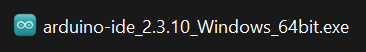
\includegraphics[width=1\linewidth]{img/chk1/1.png}
        \caption{Arduino IDE installation for Windows 11.}
        \label{fig:1}
    \end{figure}

    Once installed and opened, we needed to add support for the ESP32 board. To do this, we went to File > Preferences.
    There, we added the URL \url{https://dl.espressif.com/dl/package_esp32_index.json} in the ``Additional Boards Manager URLs'' field and clicked ``OK'', as shown in Figure~\ref{fig:2}.

    \begin{figure}[htbp]
        \centering
        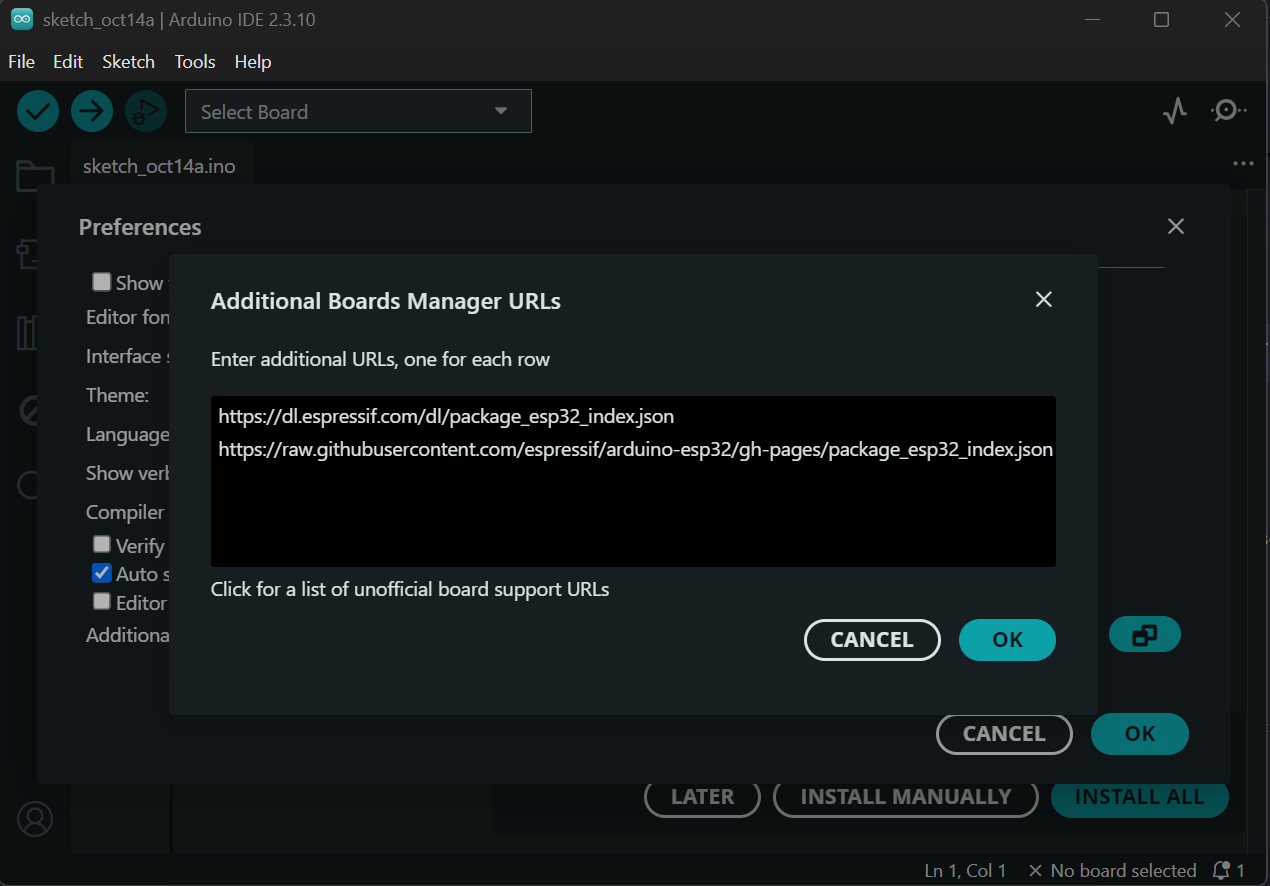
\includegraphics[width=1\linewidth]{img/chk1/2.png}
        \caption{Arduino IDE preferences with the ESP32 board manager URL added.}
        \label{fig:2}
    \end{figure}

    Then, we needed to install the board support package for the ESP32. To do this, we went to Tools > Board > Boards Manager.
    There, we searched for ``esp32'' and installed the package provided by Espressif Systems, as shown in Figure~\ref{fig:3}.

    \begin{figure}[htbp]
        \centering
        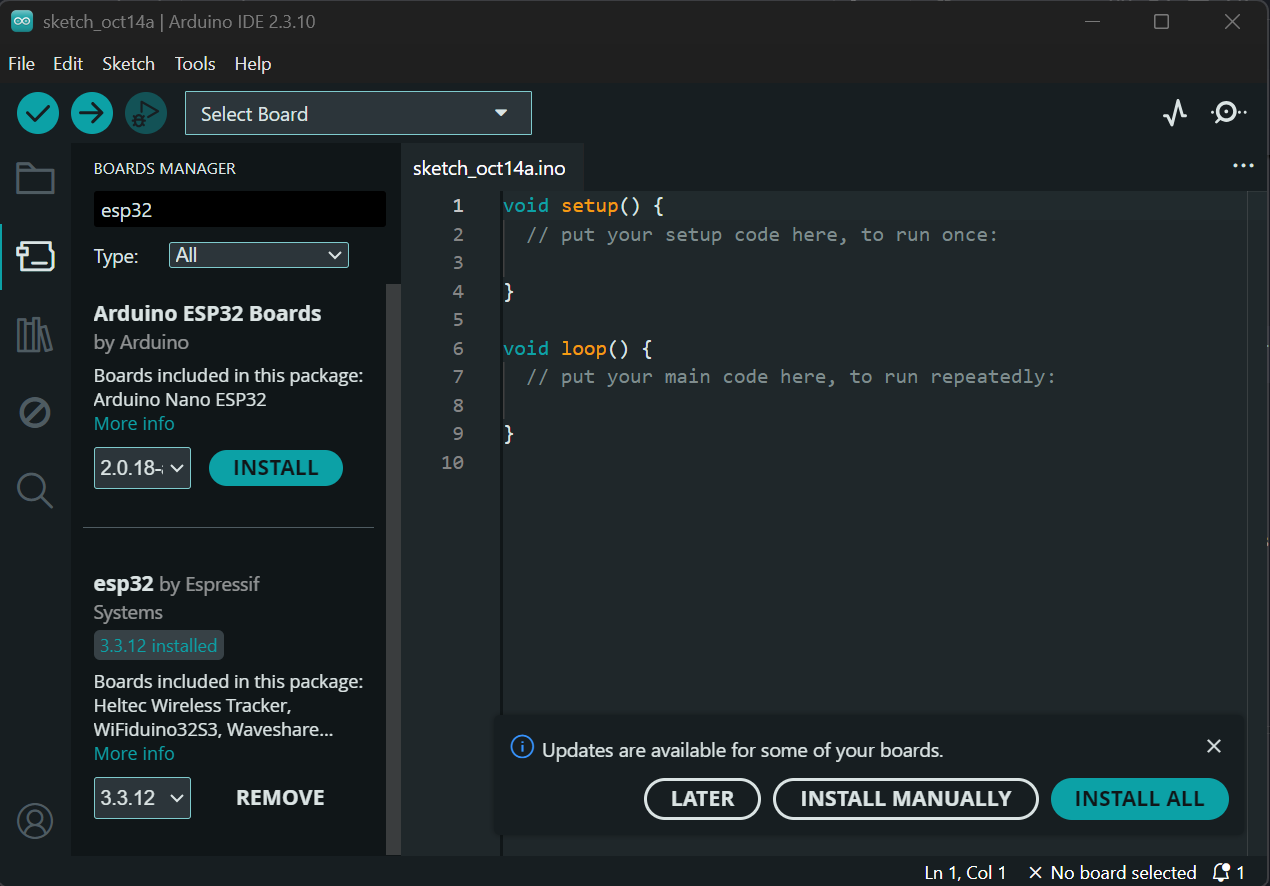
\includegraphics[width=1\linewidth]{img/chk1/3.png}
        \caption{Installation of the ESP32 board support package by Espressif Systems.}
        \label{fig:3}
    \end{figure}

    To finish the initial setup, we went to Select Board > Select Other Board and Port.
    There, we searched for ``NodeMCU-32S'' in the board selection section and selected ``COM5 Serial Port'' in the ports section, as shown in Figure~\ref{fig:4}.

    \begin{figure}[htbp]
        \centering
        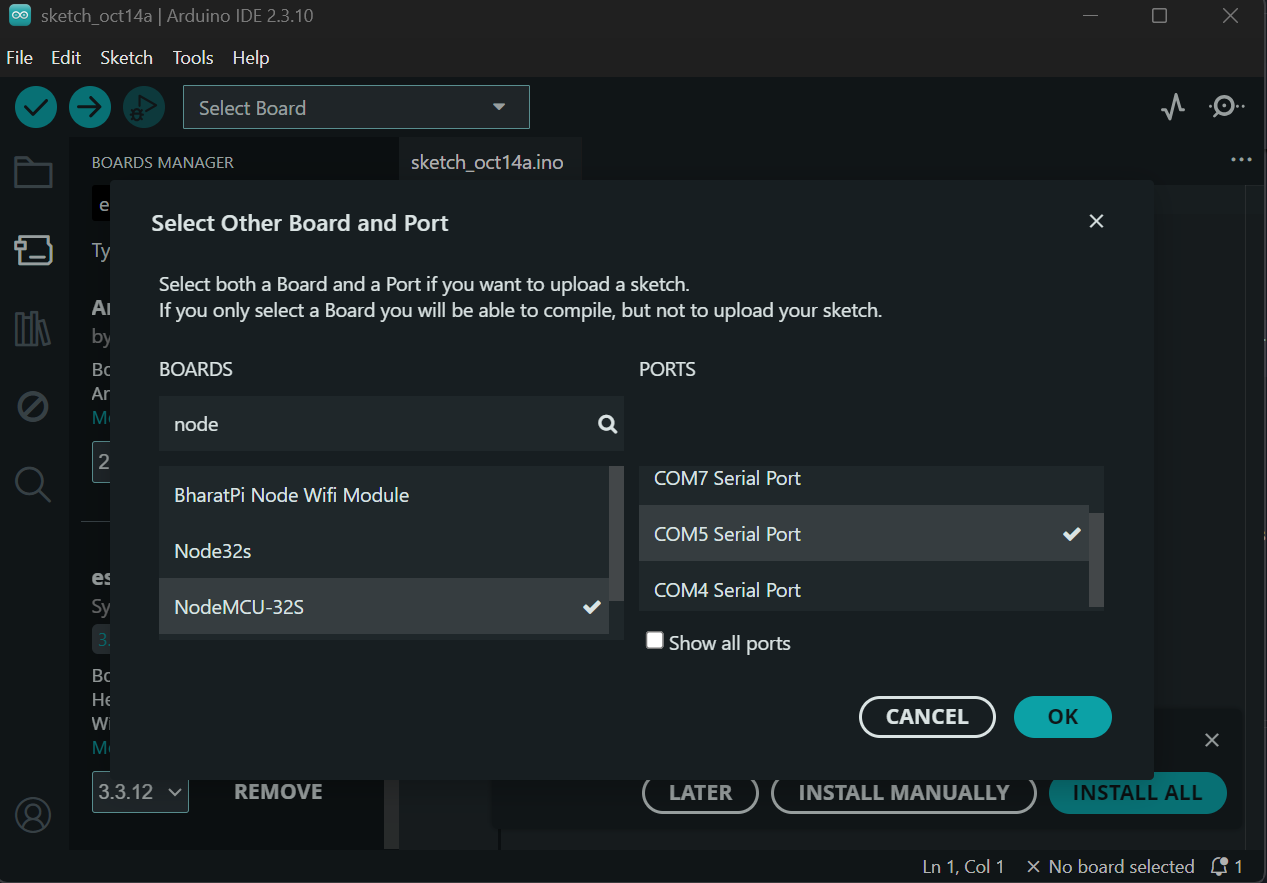
\includegraphics[width=1\linewidth]{img/chk1/4.png}
        \caption{Initial selection of the NodeMCU-32S board and COM5 serial port in Arduino IDE.}
        \label{fig:4}
    \end{figure}


    \item \textbf{Test Code Upload}

    We tested a very simple code and actually ran into a small problem during the upload process. As shown in Figure~\ref{fig:5}, there was an issue with the selected serial port.
    We solved this by changing ``COM5 Serial Port'' to ``COM3 Serial Port (USB)'', which corresponded to the connected ESP32, as shown in Figure~\ref{fig:6}.
    After fixing this issue, we successfully uploaded and ran the test code on the ESP32, as shown in Figures~\ref{fig:7} and~\ref{fig:8}.

    \begin{figure}[htbp]
        \centering
        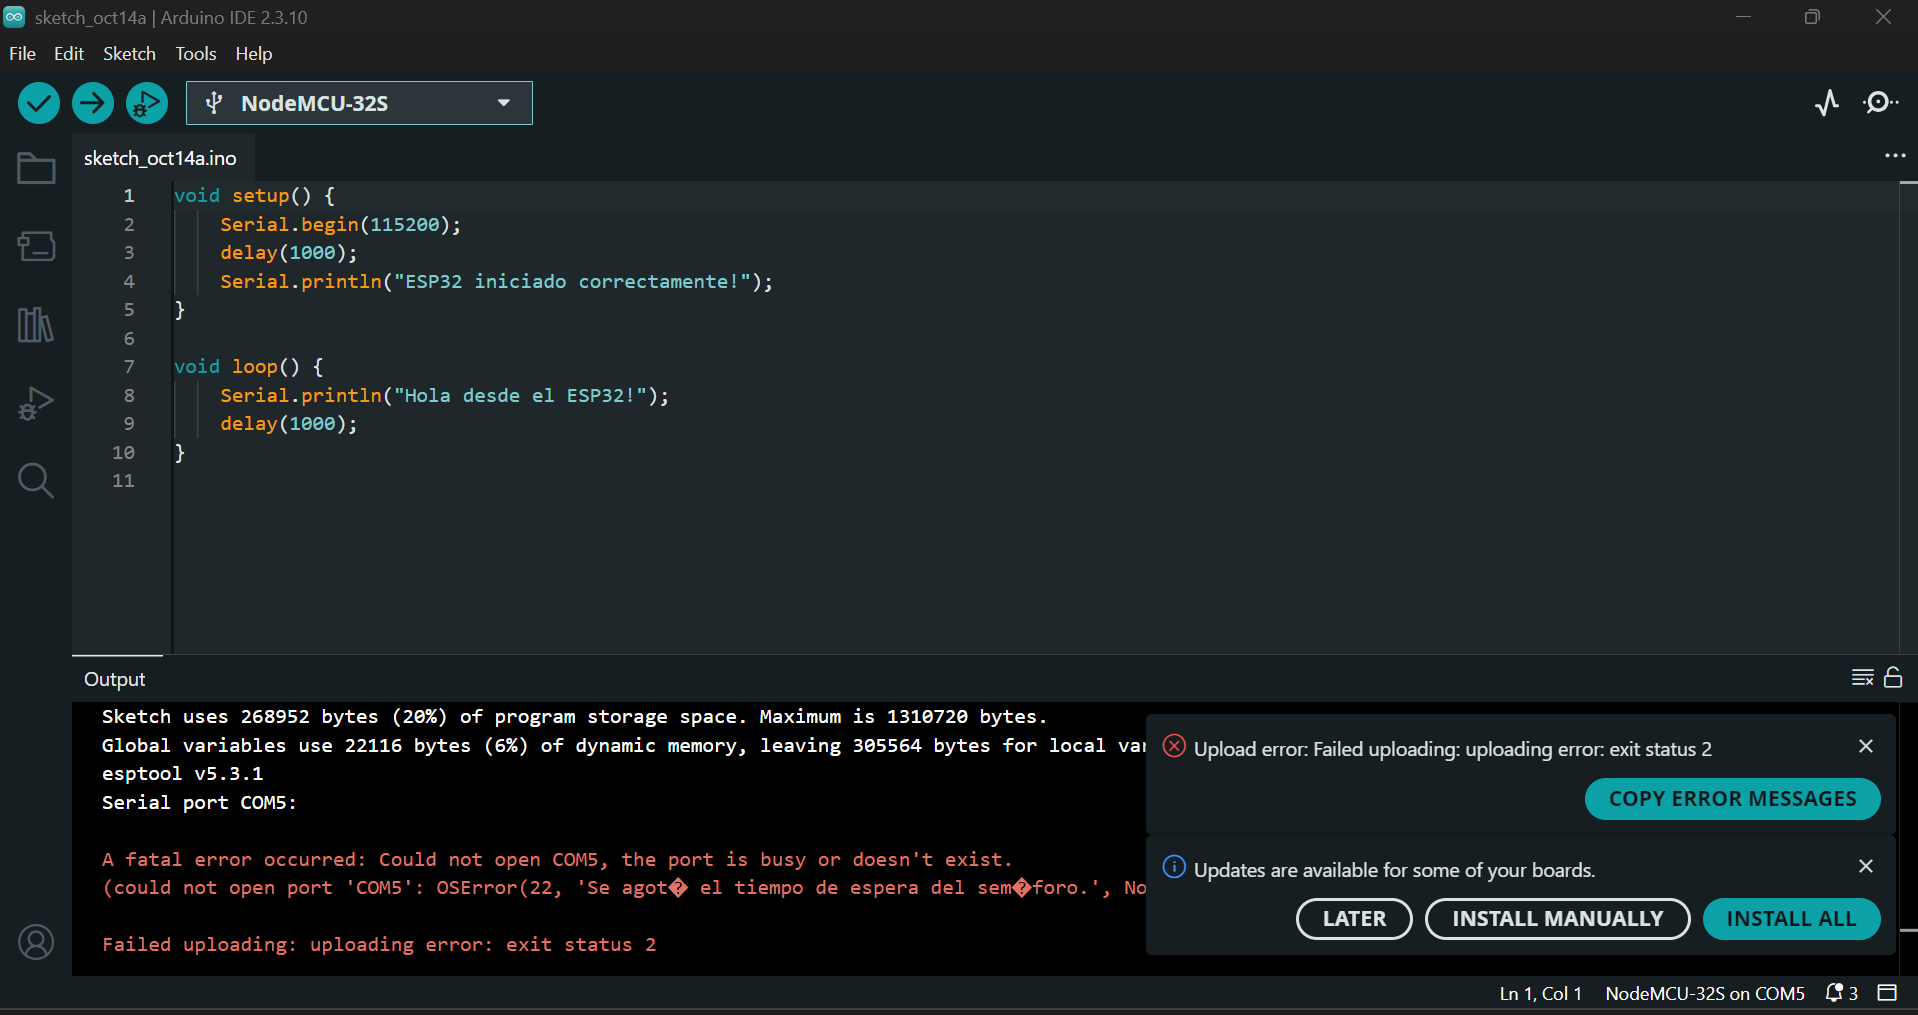
\includegraphics[width=1\linewidth]{img/chk1/5.png}
        \caption{Error encountered during the initial code upload due to the incorrect serial port selection.}
        \label{fig:5}
    \end{figure}

    \begin{figure}[htbp]
        \centering
        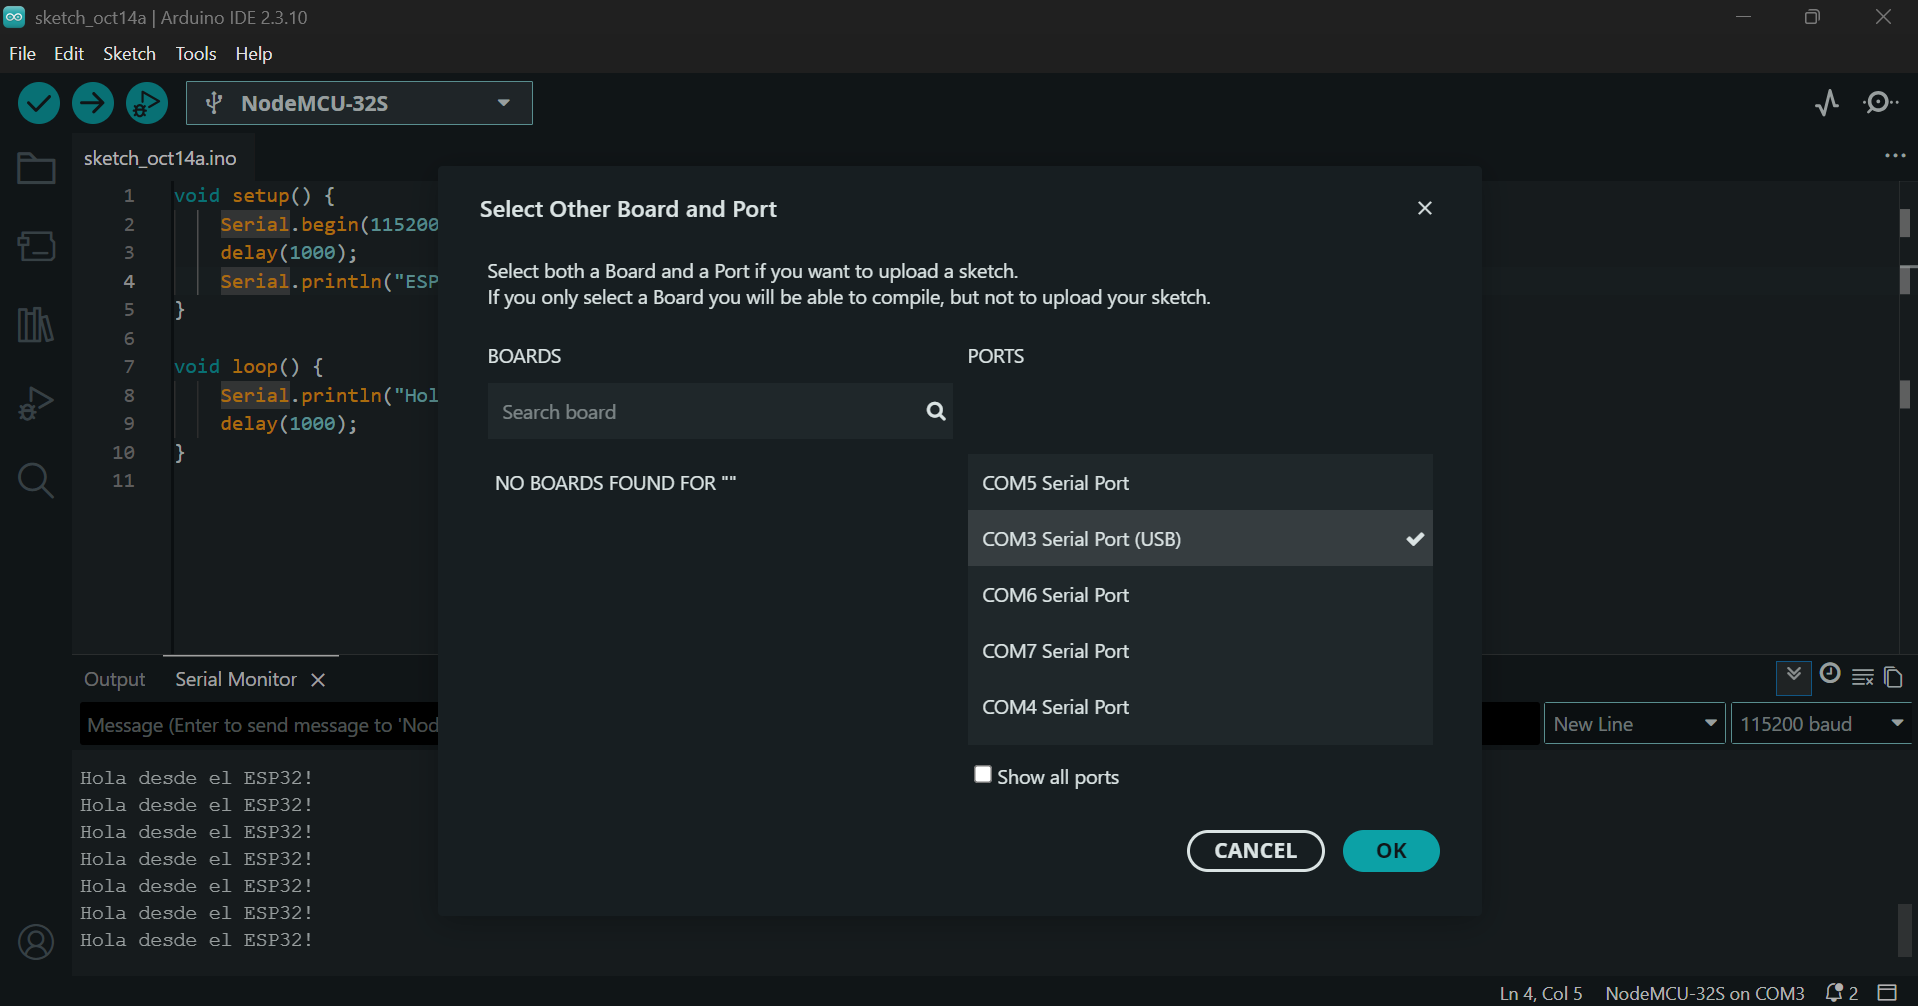
\includegraphics[width=1\linewidth]{img/chk1/6.png}
        \caption{Correction of the serial port selection from COM5 to COM3 (USB).}
        \label{fig:6}
    \end{figure}

    \begin{figure}[htbp]
        \centering
        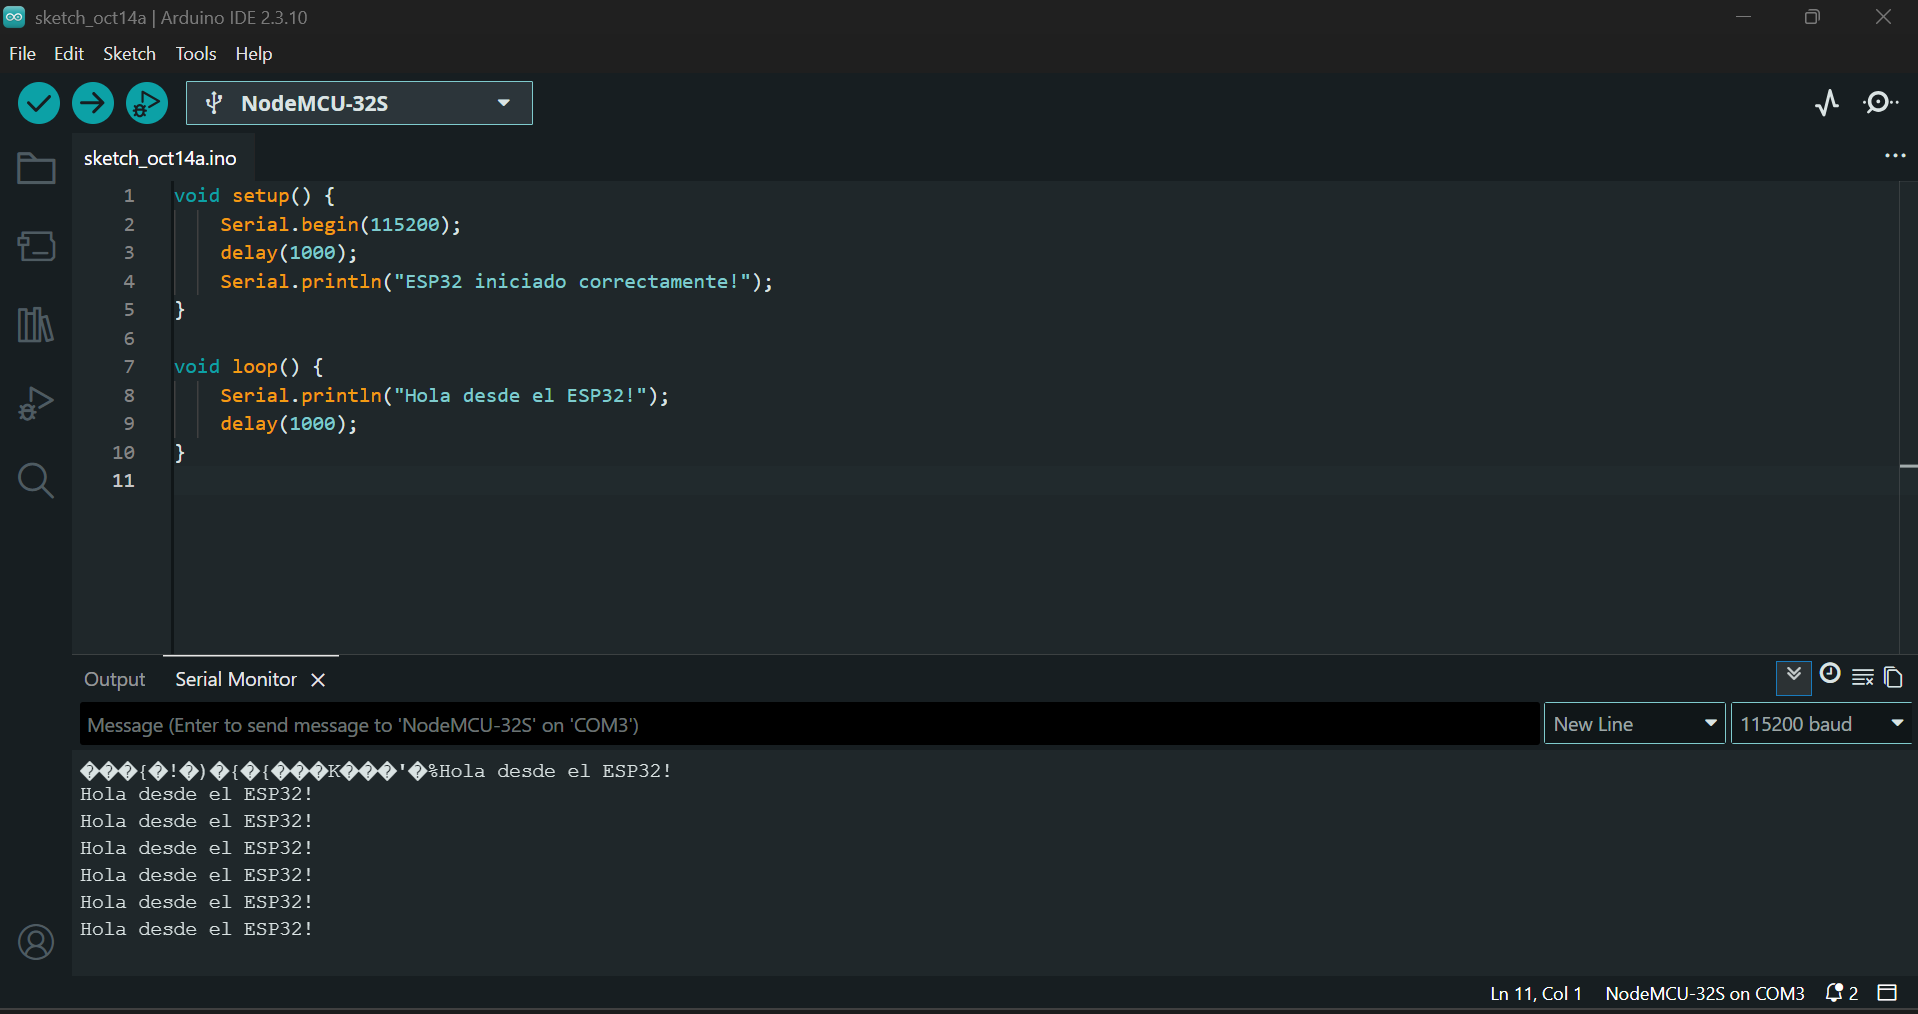
\includegraphics[width=1\linewidth]{img/chk1/7.png}
        \caption{Successful compilation and upload of the test code to the ESP32.}
        \label{fig:7}
    \end{figure}

    \begin{figure}[htbp]
        \centering
        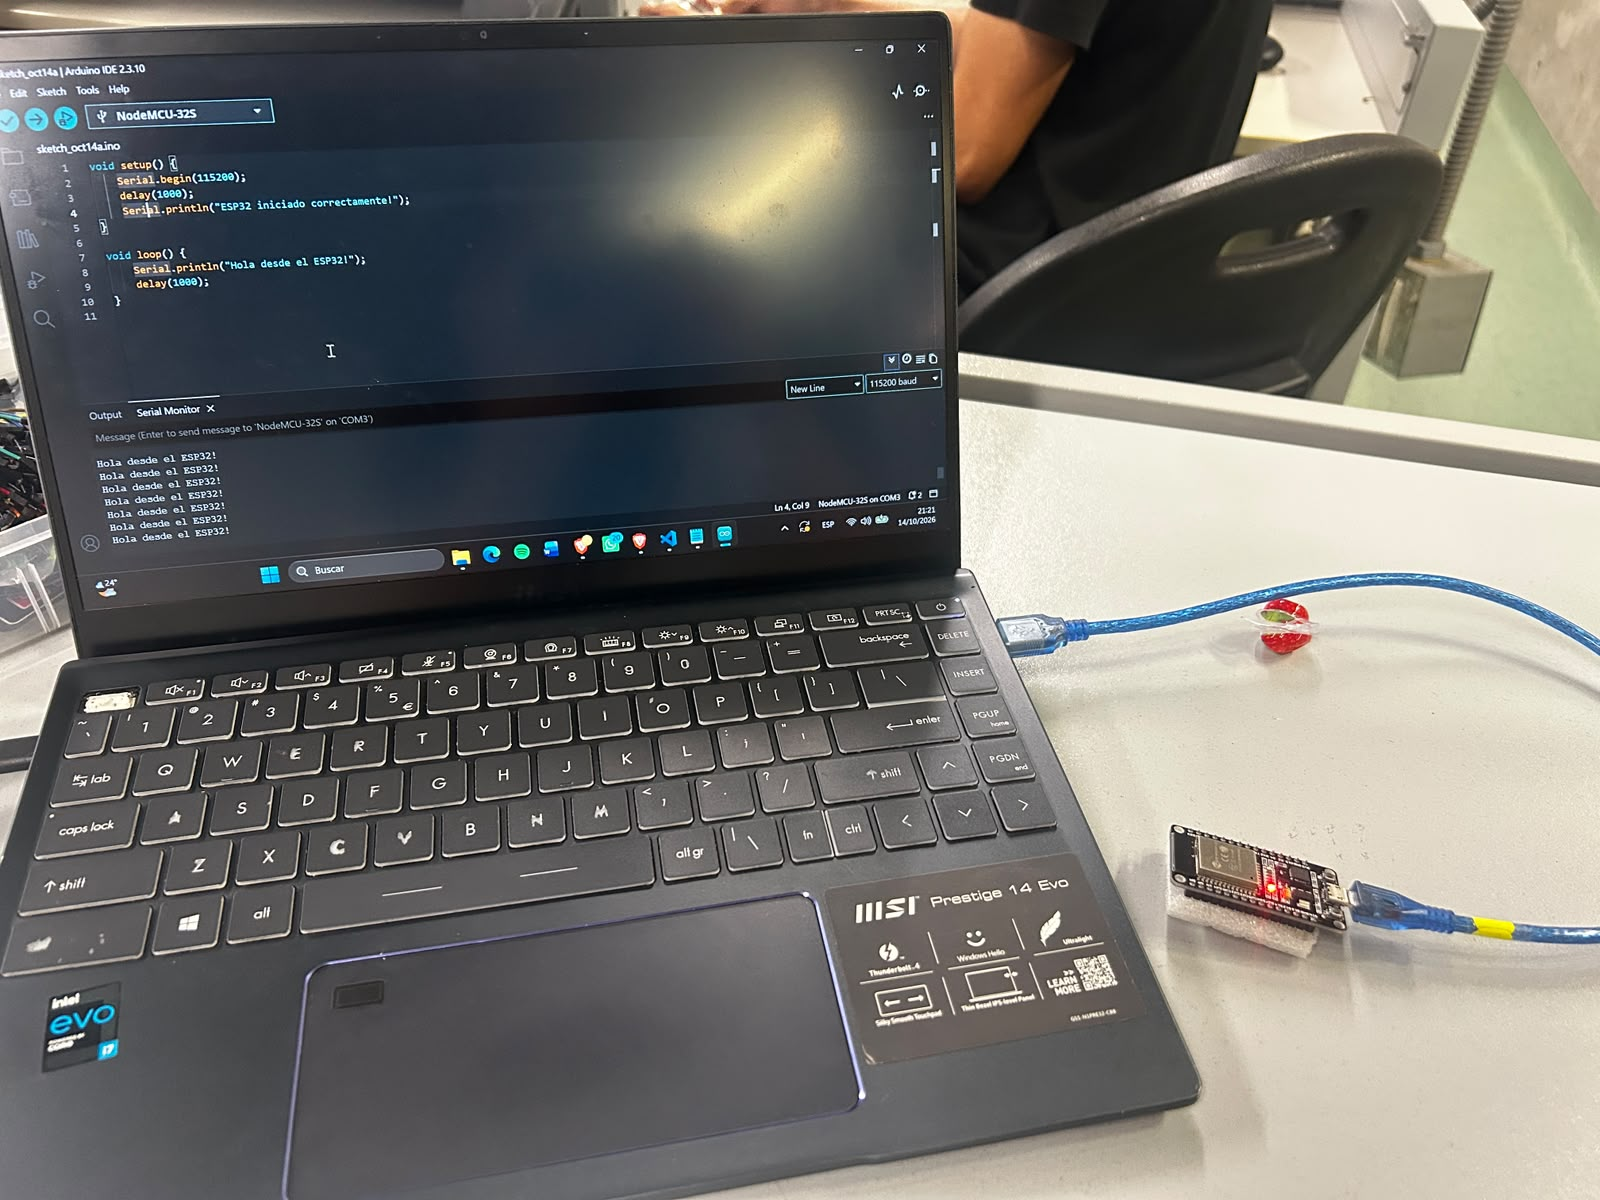
\includegraphics[width=1\linewidth]{img/chk1/8.jpeg}
        \caption{Arduino IDE Serial Monitor displaying the messages generated by the ESP32 test code.}
        \label{fig:8}
    \end{figure}


    \item \textbf{Mosquitto Installation}

    First, we downloaded the Mosquitto executable installer for Windows, as shown in Figure~\ref{fig:9}.
    As instructed, Mosquitto was installed outside the Program Files directory. We also needed to add its installation path to the system environment variables in order to execute Mosquitto commands directly from the terminal.
    We then confirmed that Mosquitto could be executed successfully, as shown in Figure~\ref{fig:10}.

    \begin{figure}[htbp]
        \centering
        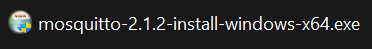
\includegraphics[width=1\linewidth]{img/chk1/9.png}
        \caption{Download of the Mosquitto installer for Windows from its official website.}
        \label{fig:9}
    \end{figure}

    \begin{figure}[htbp]
        \centering
        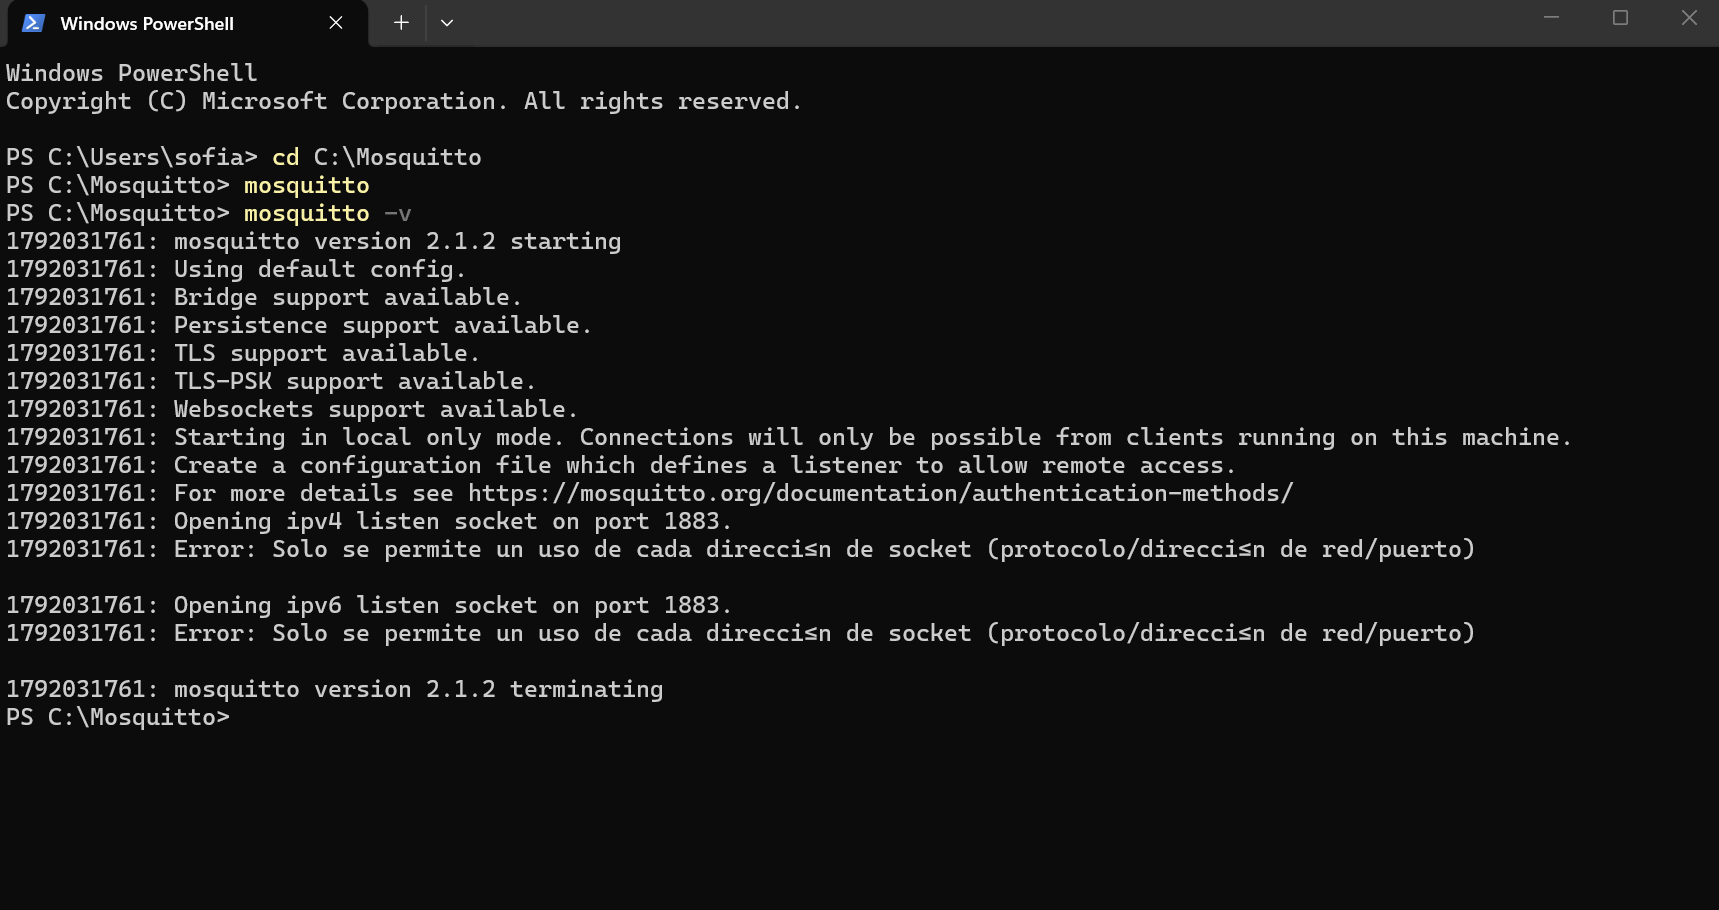
\includegraphics[width=1\linewidth]{img/chk1/10.png}
        \caption{Verification of the Mosquitto installation through the Windows terminal.}
        \label{fig:10}
    \end{figure}

    Then, we modified the Mosquitto configuration file, as shown in Figure~\ref{fig:11}, and successfully ran the broker using the updated configuration, as shown in Figure~\ref{fig:12}.

    \begin{figure}[htbp]
        \centering
        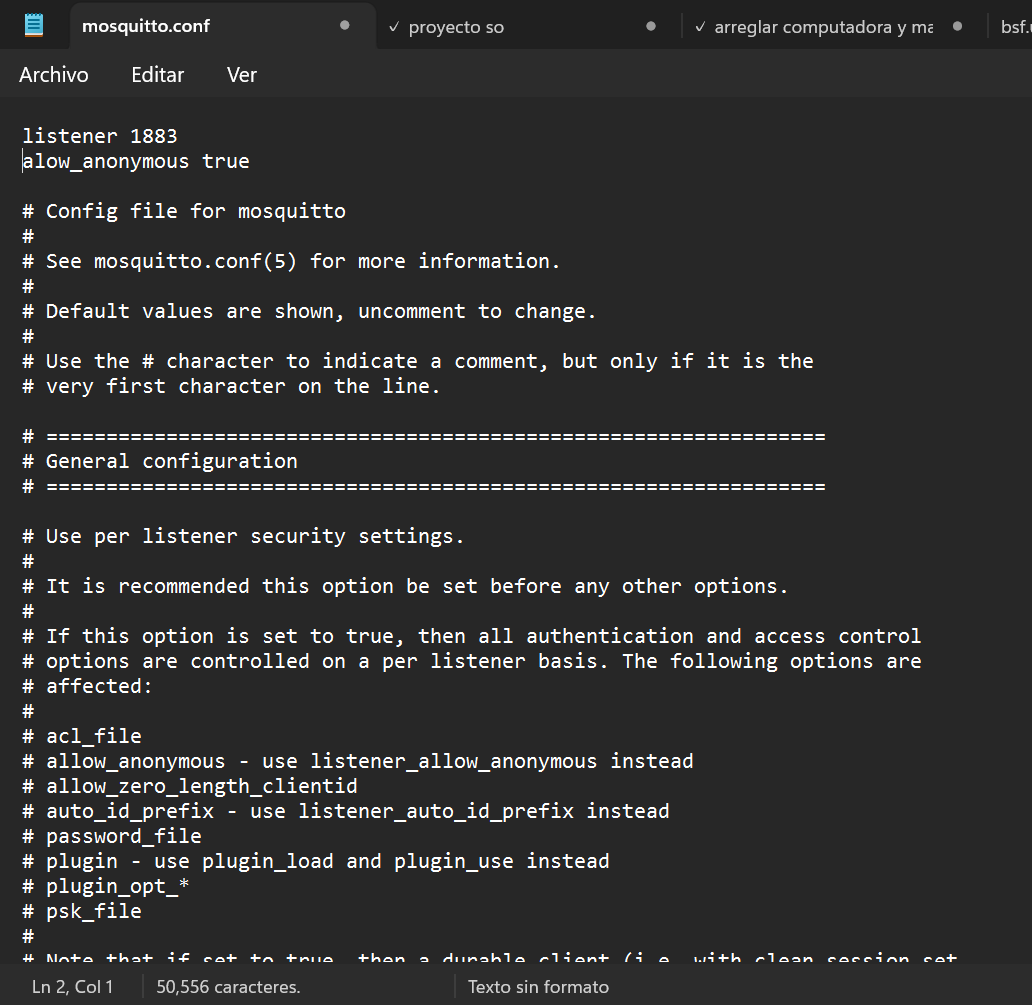
\includegraphics[width=1\linewidth]{img/chk1/11.png}
        \caption{Modification of the Mosquitto configuration file to enable connections on port 1883 and allow anonymous clients.}
        \label{fig:11}
    \end{figure}

    \begin{figure}[htbp]
        \centering
        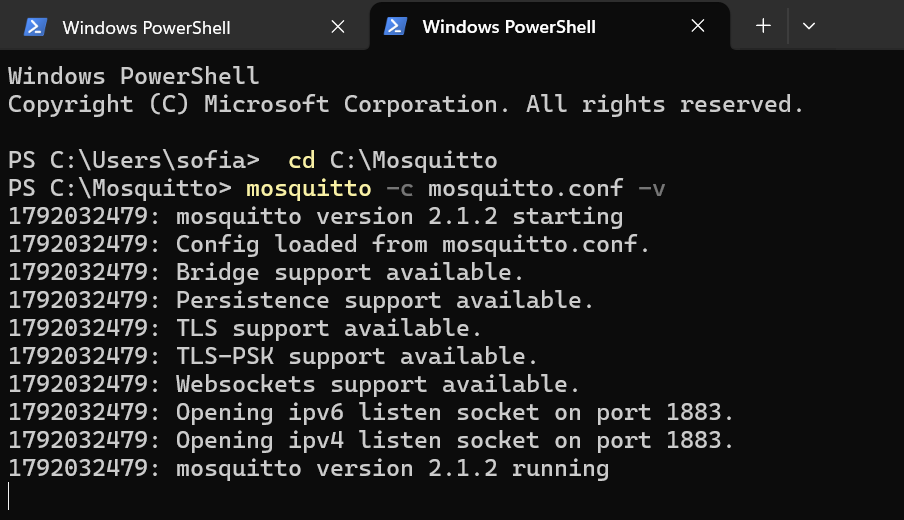
\includegraphics[width=1\linewidth]{img/chk1/12.png}
        \caption{Successful execution of the Mosquitto MQTT broker using the updated configuration file.}
        \label{fig:12}
    \end{figure}

    Finally, we tested MQTT communication by subscribing to the topic ``test/topic'' and publishing a test message to the same topic. 
    As shown in Figure~\ref{fig:14}, we published a message, and as shown in Figure~\ref{fig:13}, we were able to receive it successfully through the subscribed client.

    \begin{figure}[htbp]
        \centering
        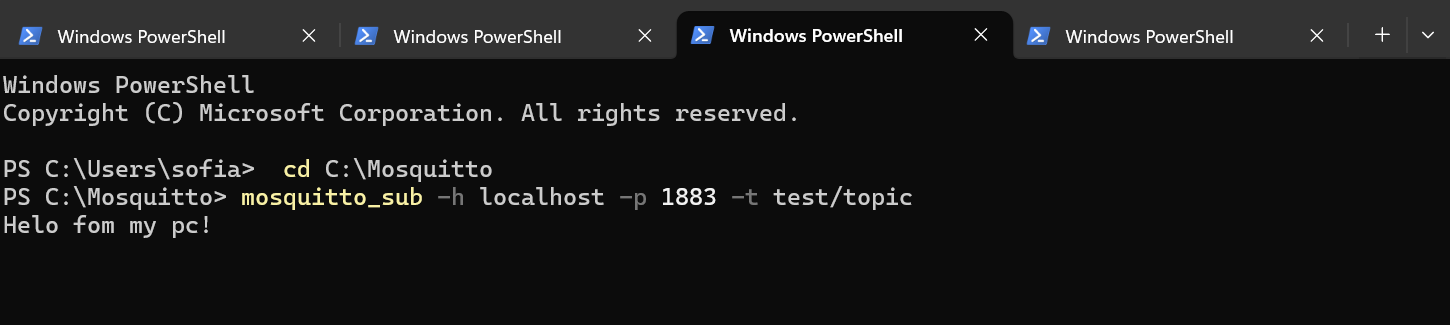
\includegraphics[width=1\linewidth]{img/chk1/13.png}
        \caption{MQTT subscriber receiving the test message through the Mosquitto broker.}
        \label{fig:13}
    \end{figure}

    \begin{figure}[htbp]
        \centering
        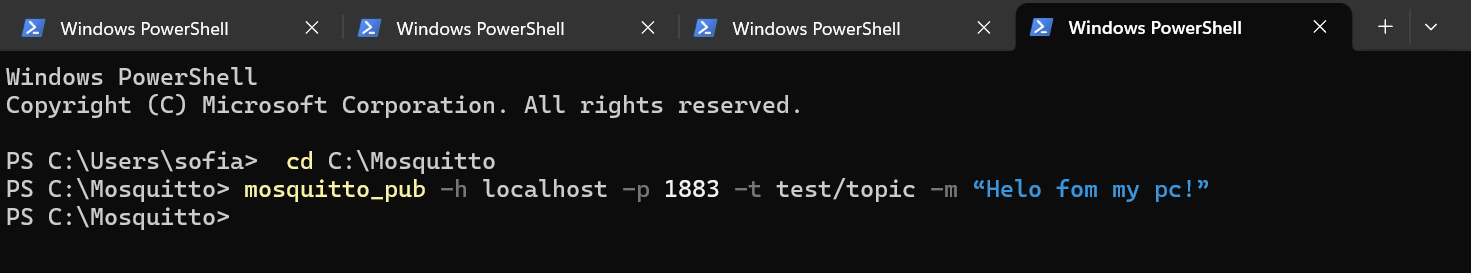
\includegraphics[width=1\linewidth]{img/chk1/14.png}
        \caption{Publication of a test message to the MQTT topic using the Mosquitto command-line client.}
        \label{fig:14}
    \end{figure}

\end{enumerate}

\subsection{CHECKPOINT 2: Basic Implementation with Reading }


\section{CConclusion}
\noindent\textit{Conclusiones y recomendaciones experimentales: por documentar.}

\bibliographystyle{IEEEtran}
\bibliography{references}
\end{document}
